\label{sec:arte_intro}
Ad oggi, sempre più libri cartacei, riviste e giornali presenti in biblioteche e archivi storici stanno venendo trasformati in versioni elettroniche che possono essere manipolate da un computer. A questo scopo, nel corso degli anni sono state sviluppate tecnologie di Optical Character Recognition (comunemente abbreviato con OCR) per tradurre le scansioni e immagini di documenti testuali in testo interpretabile e processabile da un computer. Questi sistemi, però, non sono perfetti e possono introdurre errori nel testo. Può accadere, infatti, che durante il processo di scansione alcuni caratteri vengano letti in modo errato, altri vengano aggiunti e altri ancora non riconosciuti. \E, ad esempio, particolarmente probabile che caratteri o sequenze di caratteri graficamente simili come \textit{"li"} e \textit{"n"} vengano scambiati fra di loro\cite{ocr_error_analysis}. La frequenza di tali errori è influenzata da fattori quali la condizione di deterioramento di un documento e la qualità di acquisizione dell'immagine\cite{hartley1999quality}: la presenza di granelli di polvere, caratteri scoloriti, pagine ingiallite o artefatti risultati dalla scansione, ad esempio, influiscono negativamente sulle performance dei sistemi OCR.\\
La presenza di tali errori in corpora acquisiti tramite OCR risulta problematica in quanto rende meno precisi task di Natural Language Processing (NLP) come, ad esempio, l'esecuzione di query \cite{impatto_ocr_1} o il topic modelling\cite{impatto_ocr_2}. Per ovviare a tali problemi, sono state sviluppate varie soluzioni che mirano a minimizzare il quantitativo di errori presenti nel testo estratto. \E\ possibile classificare queste soluzioni nelle seguenti due categorie:
\begin{itemize}
\item \textbf{OCR Pre-processing}: ricadono in questa categoria tutte quelle tecniche che mirano ad ottenere migliori risultati dall'estrazione del testo attraverso il miglioramento dell'input, ovvero delle immagini, che viene usato dai software di OCR. Tali metodi includono, ma non si limitano a, l'uso di migliori tecniche di scansione, la correzione del contrasto nell'immagine\cite{holley2009good} e la rotazione e correzione di deformazioni nell'immagine\cite{bieniecki2007image} (\autoref{fig:art_prep_ex}).

 
\item \textbf{OCR Post-processing}: ricadono in questa categoria tutte quelle tecniche che mirano ad individuare e correggere gli errori presenti nell'output generato dai vari software di OCR. Essendo l'OCR Post-processing oggetto di questa tesi, sarà approfondito a parte nella \autoref{sec:art_post_post}.
\end{itemize}

OCR pre-processing e post-processing sono spesso usati in congiunzione per ottenere migliori risultati dall'estrazione del testo.
\begin{figure}[H]
\centering
{
\begin{minipage}{0.35\textwidth}
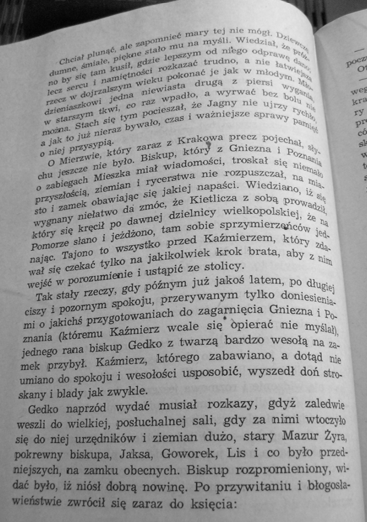
\includegraphics[width=\textwidth]{immagini/stato_arte/prep1}
\end{minipage} 
\begin{minipage}{0.06\textwidth}
\centering
\Large$\rightarrow$
\end{minipage}
\begin{minipage}{0.35\textwidth}
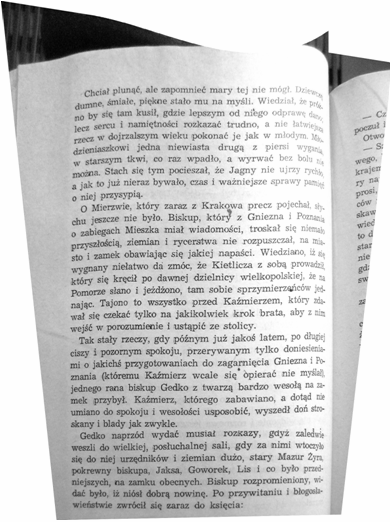
\includegraphics[width=\textwidth]{immagini/stato_arte/prep2}
\end{minipage}
\caption{A sinistra foto di una pagina contenente del testo. A destra, foto della stessa pagina pre-processata per facilitare l'estrazione del testo. Esempio preso da \cite{bieniecki2007image}.}
\label{fig:art_prep_ex}
}
\end{figure}
\noindent

\paragraph{Scopo e organizzazione della tesi} Lo svolgimento di questa tesi è consistito nello sviluppo di un sistema di OCR post-processing basato su BERT, un modello di machine learning finalizzato al Natural Language Processing sviluppata da Google. Lo sviluppo di tale sistema ha necessitato della creazione di un dataset apposito, nonché di un'adeguata metodologia di test. Il codice prodotto, che permette di replicare i risultati illustrati in questa tesi, è disponibile al seguente link:
\begin{center}
\url{https://github.com/sebacaccaro/codice_tesi}
\end{center}
\noindent
La tesi è organizzata nei seguenti capitoli:

\begin{enumerate}
\item \textbf{\nameref{sec:arte}}: in questo capitolo è definito in modo più preciso il problema dell'OCR post-processing, ed è presentata la discussione della letteratura.

\item \textbf{\nameref{sec:dataset}}: in questo capitolo si discutono le ragioni che hanno portato alla creazione di un dataset apposito, e si descrive la metodologia con la quale tale dataset è stato creato.

\item \textbf{\nameref{sec:metodologia}}: in questo capitolo si descrive la metodologia implementata dal sistema di correzione sviluppato.


\item \textbf{\nameref{sec:test}}: in questo capitolo è descritta la metodologia di test utilizzata, insieme alle metriche definite per la valutazione del sistema di correzione. Sono poi riportati e commentati i risultati dei test eseguiti


\item \textbf{\nameref{sec:analisi}}: in questo capitolo si analizzano le performance dei vari stadi del sistema di correzione, con lo scopo di capire quali fasi sono ottimizzate e quali invece hanno margini di miglioramento.
\end{enumerate}
\noindent
Sono inoltre riportate in chiusura le conclusioni tratte dai risultati e dall'analisi dell'errore, insieme ad alcuni possibili sviluppi futuri del sistema di correzione.








